\section{SCIENCE/TECHNICAL/MANAGEMENT}

%-----
% OVERVIEW
%-----

\subsection{SUBSECTION}

\subsubsection{Subsubsection}

\begin{wrapfigure}{r}{0.3\textwidth}
  \vspace{-1em}
  \noindent\small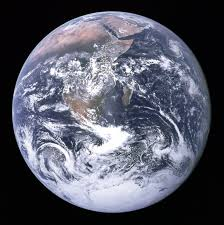
\includegraphics[width=.3\textwidth]{figures/_earth.jpg}
  \caption{<CAPTION>.}
  \vspace{-3em}
  \label{fig:_earth}
\end{wrapfigure}

\paragraph{How it works}
The Proposal main title, short title, call number and authors can be edited in the \emph{main.tex} file. 
Each main sections of the proposal (e.g. \emph{SCIENCE/TECHNICAL/MANAGEMENT}, \emph{BUDGET JUSTIFICATION}) have their own separate *.tex file. Those sections can be included in the main document by un-/commenting their related command lines in the \emph{main.tex} file. Moving those lines around also allow to change the relative location of the sections in the final document.

\paragraph{Citations} References are listed in the \emph{references.bib} file in bibtex format and can be cited within squared brackets \citep[e.g.][]{Campbell1969} or along the flow of the text like \citet{Campbell1969}.

\paragraph{Figures}
Figures can be placed across the width of the page (Fig.~\ref{fig:_mars}), or wrapped within the text with the figure on the right side of the page (Fig.~\ref{fig:_earth}). Play with the \emph{vspace} function for and after the figure to align it vertically.

\begin{figure}[thb]
 \noindent\small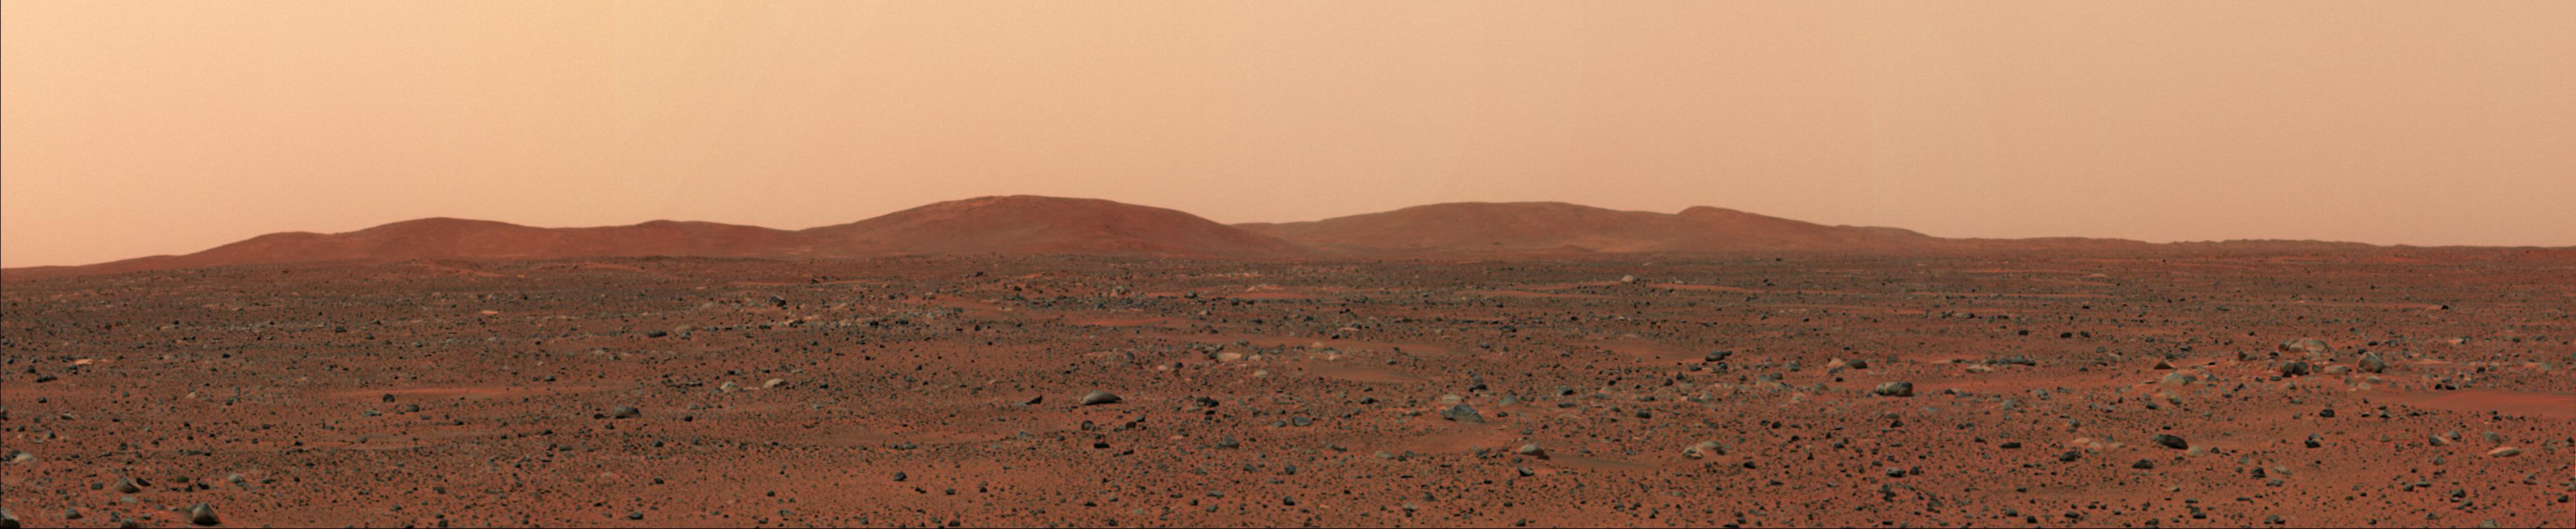
\includegraphics[width=\textwidth]{figures/_mars.jpg}
 \caption{<CAPTION>.}
 \vspace{-1em}
 \label{fig:_mars}
\end{figure}
